%%%%%%%%%%%%%%%%%%%%%%%%%%%%% Define Article %%%%%%%%%%%%%%%%%%%%%%%%%%%%%%%%%%
\documentclass{article}   % two side printing
%%%%%%%%%%%%%%%%%%%%%%%%%%%%%%%%%%%%%%%%%%%%%%%%%%%%%%%%%%%%%%%%%%%%%%%%%%%%%%%

%%%%%%%%%%%%%%%%%%%%%%%%%%%%% Using Packages %%%%%%%%%%%%%%%%%%%%%%%%%%%%%%%%%%
\usepackage{geometry}
\usepackage{graphicx}
\usepackage{amssymb}
\usepackage{amsmath}
\usepackage{amsthm}
\usepackage{empheq}
\usepackage{mdframed}
\usepackage{booktabs}
\usepackage{lipsum}
\usepackage{color}
\usepackage{psfrag}
\usepackage{pgfplots}   % For plotting beautiful graphs
\usepackage{bm}
\usepackage[spanish]{babel}
\usepackage{biblatex} 
\usepackage{csquotes} 
\usepackage{setspace}
\usepackage{multicol}  
\usepackage[skip=3pt plus 1pt, indent=30pt]{parskip}    % Setting space between paragraphs and indent
\usepackage[T1]{fontenc}    % Output font encoding for international characters
\usepackage{helvet}        % Selecting font family
\usepackage{ragged2e}      % For text alignment
\usepackage{adjustbox}       % For defining new environments
\usepackage{fancyhdr}       % For defining headers and footers
\usepackage[cochineal]{newtxmath}
\usepackage{caption}
\usetikzlibrary{intersections}
\usetikzlibrary{decorations.text}
\usetikzlibrary{decorations.pathreplacing}
%%%%%%%%%%%%%%%%%%%%%%%%%%%%%%%%%%%%%%%%%%%%%%%%%%%%%%%%%%%%%%%%%%%%%%%%%%%%%%%

% Other Settings
\newcommand*{\freq}{\mathord{\mathit{f}}}
%\let\cleardoublepage=\clearpage
%\renewcommand{\baselinestretch}{1.5}
%%%%%%%%%%%%%%%%%%%%%%%%%% Page Setting %%%%%%%%%%%%%%%%%%%%%%%%%%%%%%%%%%%%%%%
\geometry{a4paper, textwidth=19cm, textheight=28.5cm, top=0.1cm, headheight=0.1cm}  % Setting page size
\graphicspath{{images/}}    % Setting path for images
\addbibresource{bibliography.bib}   % Setting path for bibliography
%%%%%%%%%%%%%%%%%%%%%%%%%% Define some useful colors %%%%%%%%%%%%%%%%%%%%%%%%%%
\definecolor{ocre}{RGB}{243,102,25}
\definecolor{mygray}{RGB}{243,243,244}
\definecolor{deepGreen}{RGB}{26,111,0}
\definecolor{shallowGreen}{RGB}{235,255,255}
\definecolor{deepBlue}{RGB}{61,124,222}
\definecolor{shallowBlue}{RGB}{235,249,255}
%%%%%%%%%%%%%%%%%%%%%%%%%%%%%%%%%%%%%%%%%%%%%%%%%%%%%%%%%%%%%%%%%%%%%%%%%%%%%%%

%%%%%%%%%%%%%%%%%%%%%%%%%% Define an orange box command %%%%%%%%%%%%%%%%%%%%%%%%
\newcommand\orangebox[1]{\fcolorbox{ocre}{mygray}{\hspace{1em}#1\hspace{1em}}}
%%%%%%%%%%%%%%%%%%%%%%%%%%%%%%%%%%%%%%%%%%%%%%%%%%%%%%%%%%%%%%%%%%%%%%%%%%%%%%%

%%%%%%%%%%%%%%%%%%%%%%%%%%%% English Environments %%%%%%%%%%%%%%%%%%%%%%%%%%%%%
\newtheoremstyle{mytheoremstyle}{3pt}{3pt}{\normalfont}{0cm}{\rmfamily\bfseries}{}{1em}{{\color{black}\thmname{#1}~\thmnumber{#2}}\thmnote{\,--\,#3}}
\newtheoremstyle{myproblemstyle}{3pt}{3pt}{\normalfont}{0cm}{\rmfamily\bfseries}{}{1em}{{\color{black}\thmname{#1}~\thmnumber{#2}}\thmnote{\,--\,#3}}
\theoremstyle{mytheoremstyle}
\newmdtheoremenv[linewidth=1pt,backgroundcolor=shallowGreen,linecolor=deepGreen,leftmargin=0pt,innerleftmargin=20pt,innerrightmargin=20pt,]{theorem}{Theorem}[section]
\theoremstyle{mytheoremstyle}
\newmdtheoremenv[linewidth=1pt,backgroundcolor=shallowBlue,linecolor=deepBlue,leftmargin=0pt,innerleftmargin=20pt,innerrightmargin=20pt,]{definition}{Definition}[section]
\theoremstyle{myproblemstyle}
\newmdtheoremenv[linecolor=black,leftmargin=0pt,innerleftmargin=10pt,innerrightmargin=10pt,]{problem}{Problem}[section]
%%%%%%%%%%%%%%%%%%%%%%%%%%%%%%%%%%%%%%%%%%%%%%%%%%%%%%%%%%%%%%%%%%%%%%%%%%%%%%%

%%%%%%%%%%%%%%%%%%%%%%%%%%%%%%% Plotting Settings %%%%%%%%%%%%%%%%%%%%%%%%%%%%%
\usepgfplotslibrary{colorbrewer}
\pgfplotsset{width=8cm,compat=1.9}
%%%%%%%%%%%%%%%%%%%%%%%%%%%%%%%%%%%%%%%%%%%%%%%%%%%%%%%%%%%%%%%%%%%%%%%%%%%%%%%

%%%%%%%%%%%%%%%%%%%%%%%%%%%%%%% Title & Author %%%%%%%%%%%%%%%%%%%%%%%%%%%%%%%%
\title{Análisis de parámetros de dispersión en una microcinta}
\author{Luis Guillermo Macias Rojas}
%%%%%%%%%%%%%%%%%%%%%%%%%%%%%%%%%%%%%%%%%%%%%%%%%%%%%%%%%%%%%%%%%%%%%%%%%%%%%%%

%%%%%%%%%%%%%%%%%%%%%%%%%%%%%%% Header & Footer %%%%%%%%%%%%%%%%%%%%%%%%%%%%%%%
\pagestyle{fancy}  % Setting page style
\fancyhf{}
\fancyhead[L]{\text{Luis Guillermo Macias Rojas}}  % Setting header
%%%%%%%%%%%%%%%%%%%%%%%%%%%%%%%%%%%%%%%%%%%%%%%%%%%%%%%%%%%%%%%%%%%%%%%%%%%%%%%

\begin{document}
    \maketitle

    \fontfamily{phv}\selectfont % Selecting font family
    \noindent
    \textbf{Resumen:} En este trabajo se presenta un estudio comparativo de los parámetros $S_{11}$ (reflexión) y $S_{21}$ (transmisión)
    de una microcinta diseñada para operar a 10 GHz entre dos metodologías de simulación: Una basada en el
    modelado electromagnético de onda completa en Ansys HFSS, que resuelve las ecuaciones de Maxwell de forma rigurosa, y
    otra utilizando la herramienta ADS (Advanced Design System) de Keysight, que emplea modelos analíticos y aproximaciones
    cuasi-estáticas para caracterizar la microcinta. Para el modelado del substrato se utilizó un dieléctrico TerraGreen 400G (RF/MW)
    de Isola Group con una constante dieléctrica de 3.15 y un espesor de 0.254 mm.

    \noindent\begin{minipage}{0.49\textwidth}   %uses 60% of the page
        {\centering\section*{\large Introducción}}

        En el diseño de circuitos de alta frecuencia, el análisis de parámetros de dispersión (parámetros S) es fundamental para
        evaluar el desempeño de estructuras como líneas de microcinta. Estos parámetros, en particular $S_{11}$ (pérdida por retorno)
        y $S_{21}$ (pérdida por inserción), permiten cuantificar las reflexiones y atenuaciones de la señal en función de la
        frecuencia, aspectos críticos para garantizar la integridad de la señal y la eficiencia energética en aplicaciones como
        antenas, filtros y diseño de PCBs.
        
        {\centering\section*{\large Metodología}}

        La matriz de dispersión \eqref{s_matrix} describe el comportamiento de redes eléctricas mediante el
        análisis de ondas incidentes, reflejadas y transmitidas en sus puertos. A diferencia de los parámetros absolutos, como
        los de impedancia (Z) o los ABCD —que caracterizan propiedades intrínsecas del circuito, como voltajes y corrientes en
        terminales—, los parámetros S son relativos y dependen de la impedancia utilizada
        como referencia ($Z_0$).

        \begin{equation}
            \begin{bmatrix}
                b_1\\
                b_2
            \end{bmatrix}
            =
            \begin{bmatrix}
                S_{11} & S_{12}\\
                S_{21} & S_{22}
            \end{bmatrix}
            \cdot
            \begin{bmatrix}
                a_1\\
                a_2
            \end{bmatrix}
            \label{s_matrix}
        \end{equation}

        En redes eléctricas pasivas de dos puertos y diseñadas como la línea de microcinta en cuestión, los parámetros S cumplen con las
        propiedades de reciprocidad \eqref{eq:reciprocidad} y simetría \eqref{eq:simetria}. Esto implica que al caracterizar $S_{11}$
        y $S_{21}$, los valores de $S_{22}$ y $S_{12}$ quedan automáticamente determinados.

        \begin{equation}
            S_{12}=S_{21}
            \label{eq:reciprocidad}
        \end{equation}

        \begin{equation}
            S_{22}=S_{11}
            \label{eq:simetria}
        \end{equation}

        La estructura de microcinta se diseñó en HFSS con el objetivo de obtener 50 $\Omega$ en $Z_0$. Para ello se
        establecieron los siguientes parámetros con ayuda de la hoja de datos del fabricante del sustrato TerraGreen 400G (RF/MW):
        
        \vspace{5 mm}

        \begin{itemize}
            \item Permitividad relativa del dieléctrico: 3.15
            \item Ancho de la microcinta: 0.6 mm
            \item Largo de la microcinta: 37.9 mm
            \item Espesor del sustrato: 0.254 mm
            \item Espesor del cobre: 17.4 $\mu$m
        \end{itemize}

        \vspace{5 mm}

        Una vez simulada la estructura de microcinta en HFSS, se exportaron los parámetros S para compararlos con los
        obtenidos mediante un modelo de microcinta en ADS.
    \end{minipage}
    \hspace{0.38 cm}
    \begin{minipage}{0.49\textwidth}   %uses 40% of the page
        {\centering\section*{\large Resultados}}

        Los resultados de las simulaciones en HFSS y ADS se presentan en las figuras \ref{fig:s11} y \ref{fig:s21}. La primera
        muestra la pérdida por retorno $S_{11}$ en función de la frecuencia, mientras que la segunda presenta la pérdida por
        inserción $S_{21}$. En ambos casos, se observa una buena concordancia entre las simulaciones, con una diferencia
        máxima de 3.5 dB en $S_{11}$ y 0.8 dB en $S_{21}$.

        
        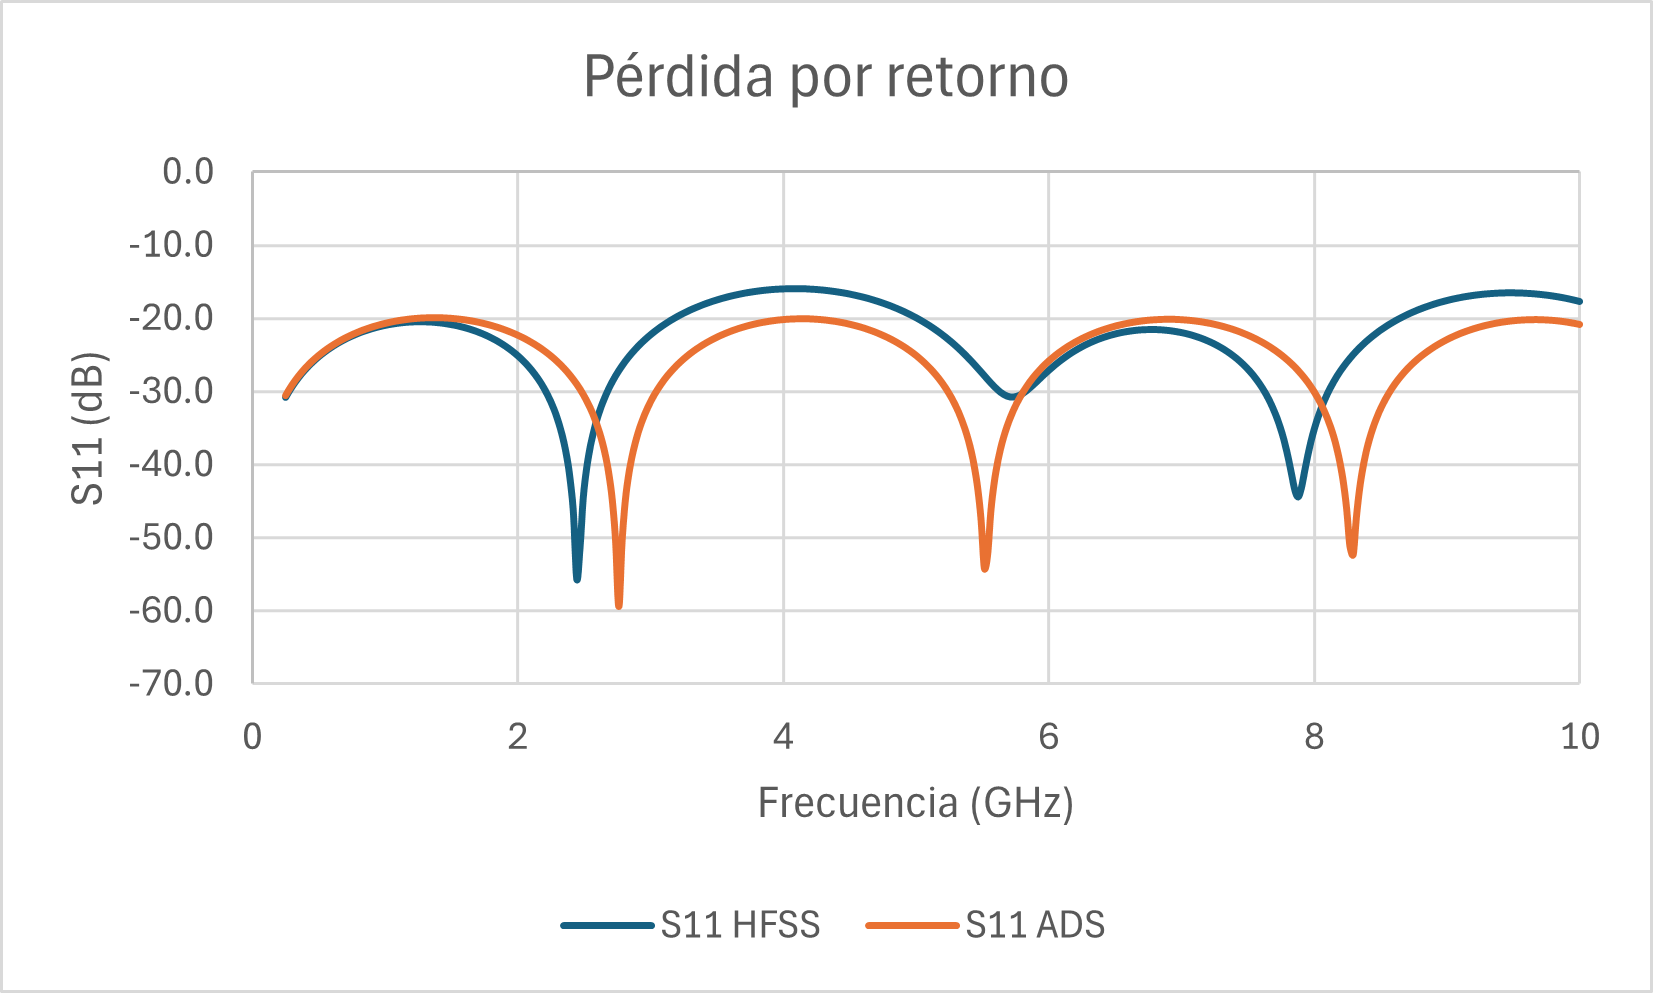
\includegraphics[width=\textwidth]{figures/s11.png}
        \captionof{figure}{Pérdida por retorno $S_{11}$ en función de la frecuencia.}
        \label{fig:s11}

        \vspace{5 mm}

        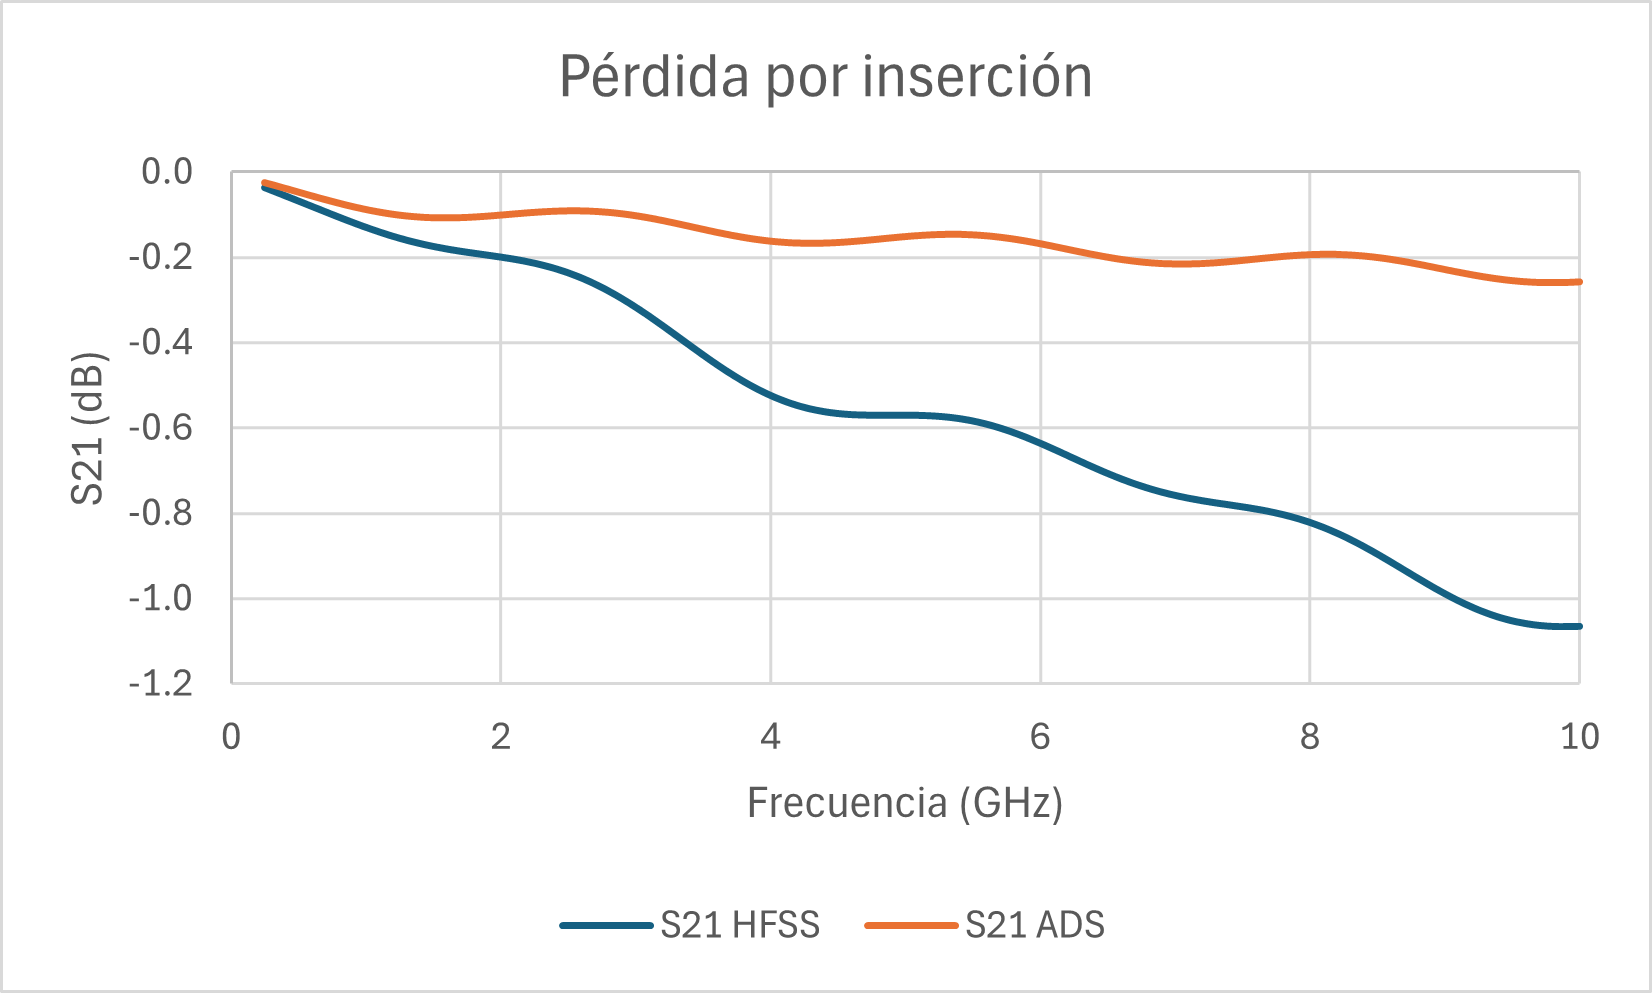
\includegraphics[width=\textwidth]{figures/s21.png}
        \captionof{figure}{Pérdida por inserción $S_{21}$ en función de la frecuencia.}
        \label{fig:s21}
        
        {\centering\section*{\large Conclusiones}}

        El análisis comparativo de los parámetros de dispersión de una microcinta en HFSS y ADS permitió validar la
        aproximación analítica de la herramienta ADS para el diseño de estructuras en alta frecuencia. La buena concordancia
        entre ambas metodologías sugiere que el modelo de microcinta en ADS ofrece una buena aproximación al simulador de onda
        completa de HFSS, especialmente para $S_{11}$.
    \end{minipage}
    %\printbibliography  % Print bibliography
\end{document}